\section{Fourier Series}
\indent The Fourier Series expresses periodic functions as 
sums of weighted cosine and sine functions of different frequencies, 
where the frequencies are integer multiples of the base frequency (frequency of the periodic function).
Every non constant term in the Fourier Series are defined as 
a coefficient multiplied by a cosine or sine function of a frequency.



\subsection{Evaluation of Constants and Coefficients}
\indent However, most of the time, we only have some information about the function, 
and we are required to construct the Fourier Series for the function. 
The major challenge is to find out the coefficients for every frequencies in order to do so.

\indent The general formula of the Trigonometric Fourier Series can be written as
\begin{equation}
    f(t) = a_0 + \sum_{n=1}^{\infty}a_n\cos(\frac{2n\pi t}{T}) + \sum_{n=1}^{\infty}b_n\sin(\frac{2n\pi t}{T})
    \label{equ:trig_fourier_series_expansion}
\end{equation}
, where $T$ is the period of $f(t)$, and $n\in\mathbb{Z}$.

\indent For a periodic function $f(t)$ with a period of $T$, 
we noticed that taking the definite integral of $f(t)$ from the start of a cycle to the end of the cycle
then divided by the period (length of a cycle) gives the average value of $f(t)$. 
$$  
    \frac{1}{T}     \int_{T}f(t)\mathrm{d}t
    = \frac{1}{T}   \int_{T}a_0\mathrm{d}t
    + \frac{1}{T}   \sum_{n=1}^{\infty}   a_n   \int_{T}\cos(\frac{2n\pi t}{T})\mathrm{d}t
    + \frac{1}{T}   \sum_{n=1}^{\infty}   b_n \int_{T}\sin(\frac{2n\pi t}{T})\mathrm{d}t
$$
Evaluate the definite integrals on the right side of the equation:
$$      \int_{T} a_0 \mathrm{d}t    =   a_0  T                  $$
$$      \int_{T}\cos(\frac{2n\pi t}{T})\mathrm{d}t  = 0         $$
$$      \int_{T}\sin(\frac{2n\pi t}{T})\mathrm{d}t  = 0         $$

We sub in the results into the equation and simplify it to get:
\begin{equation}
    a_0  =  \frac{1}{T} \int_{T} f(t) \mathrm{d}t
    \label{equ:fourier_series_a0_term}
\end{equation}


\indent Using this method, we get the average of the periodic function, 
or in other words the term we evaluated the term $a_0$. However, 
we still have to find a way to calculate the rest of the coefficients.
Before doing so, we have to know some knowledge about definite integrals of cosine and sine functions. 
For any constant $a_0$ and integers $m$ and $n$ where $m\not=n$:
$$      \int_{2\pi} a_0\cos(mx) \mathrm{d}x    =   0            $$
$$      \int_{2\pi} a_0\sin(mx) \mathrm{d}x    =   0            $$
$$      \int_{2\pi} \cos(mx)\sin(nx) \mathrm{d}x    =   0       $$
$$      \int_{2\pi} \cos(mx)\cos(nx) \mathrm{d}x    =   0       $$
$$      \int_{2\pi} \sin(mx)\sin(nx) \mathrm{d}x    =   0       $$
$$      \int_{2\pi} \cos(mx)\sin(mx) \mathrm{d}x    =   0       $$
$$      \int_{2\pi} \cos^2(mx) \mathrm{d}x    =   \pi           $$
$$      \int_{2\pi} \sin^2(mx) \mathrm{d}x    =   \pi           $$
\indent From the above equations, we know that multiplying a cosine or sine function by 
another cosine or sine function of a different frequency before taking the definite integral 
does not have a influence on the result. The exception is that when it is multiplied by itself, 
the result changes from $0$ to $\pi$. This is useful, 
we can multiply $f(t)$ by the desired cosine or sine function that contains the desired frequency 
to get the corresponding coefficient of the term.
\begin{equation}
    a_n =   \frac{2}{T} \int_{T} f(t)\cos(\frac{2n\pi t}{T}) \mathrm{d}t
    \label{equ:trig_fourier_series_cosine_coeff}
\end{equation}
\begin{equation}
    b_n =   \frac{2}{T} \int_{T} f(t)\sin(\frac{2n\pi t}{T}) \mathrm{d}t
    \label{equ:trig_fourier_series_sine_coeff}
\end{equation}








\subsection{Fourier Spectrum}
Since a periodic function can be expressed as a Fourier Series, 
we can use a spectrum to defined a Fourier Series where the x-value would be the frequency of the term instead of time,
and the y-value could be the corresponding amplitude/coefficient of the term 
or the corresponding phase shift of the term. 








\subsubsection{Single-Sided Spectra}
In equation (\ref{equ:trig_fourier_series_expansion}), there are four parameters we have to figure out, 
which is a lot of calculation. We can reduce them, since the sum of cosine and sine function of the same frequency 
can be expressed in one single term of cosine or sine function using the Sum-to-Product Identities. 
This would add an extra parameter, phase shift into the equation, 
however, it removes the amplitude of cosine or sine function, and the corresponding frequency. 
After combining the cosine terms and the sine terms into only cosine or sine terms, 
every term in the trigonometric form of a periodic function can be described using 
three parameters: amplitude, frequency and phase shift. 
Let $\omega_0$ be the base frequency, and $\omega_0=\frac{2\pi}{T}$.
This can be proved. From (\ref{equ:trig_fourier_series_expansion}), 
we can combine the cosine and sine functions that has the same frequency together into one single term, 
because a cosine function added to a sine function is a shifted, compressed or stretched cosine or sine function.
Let $C_0 = D_0 = a_0$ we obtain the compacted form of the Fourier Series:

\begin{equation}
    f(t) =      C_0     +   \sum_{n=1}^{\infty} C_n \cdot \cos(n\omega_0t+\phi_n)
    \label{equ:fourier_spectrum_cosine}
\end{equation}
\begin{equation}
    f(t) =      D_0     +   \sum_{n=1}^{\infty} D_n \cdot \sin(n\omega_0t+\theta_n)
    \label{equ:fourier_spectrum_sine}
\end{equation}

$n\omega_0$ in this equation is the frequency of each term, 
$C_n$ and $D_n$ are the amplitudes of the corresponding frequency,
and $\phi_n$ is the corresponding phase shift. Both (\ref{equ:fourier_spectrum_cosine}) 
and (\ref{equ:fourier_spectrum_sine}) would work, 
but (\ref{equ:fourier_spectrum_cosine}) is preferred most of the times. 
We would use (\ref{equ:fourier_spectrum_cosine}) in this subsection.

This concept can be proved algebraically. 
$$\begin{aligned}
f(t) &= C_0  +  \sum_{n=1}^{\infty} C_n \cdot \cos(n\omega_0t+\phi_n)   \\
&= C_0  +  \sum_{n=1}^{\infty} C_n \left[ \cos(n\omega_0t)\cos(\phi_n) - \sin(n\omega_0t)\sin(\phi_n) \right]   \\
&= C_0  +  \sum_{n=1}^{\infty} C_n \cos(n\omega_0t)\cos(\phi_n) - \sum_{n=1}^{\infty} C_n \sin(n\omega_0t)\sin(\phi_n)
\end{aligned}$$

Compare the coefficients of the above equation with (\ref{equ:trig_fourier_series_expansion}), we get:
\begin{equation}
    \begin{cases}
        a_0     =       C_0                 \\
        a_n     =       C_n\cos(\phi_n)     \\
        b_n     =       -C_n\sin(\phi_n)
    \end{cases}
    \label{equ:an_bn_with_Cn_relationship}
\end{equation}

Compute $a_n^2 + b_n^2$ using ({\ref{equ:an_bn_with_Cn_relationship}}) would gives the first equation below, 
and divide $b_n$ by $a_n$ gives the second equation below, we obtain:
\begin{equation} \begin{cases}
    C_0 = a_0       \\
    C_n^2     =       a_n^2     +       b_n^2       \\
    \tan(\phi_n)   =    -\frac{b_n}{a_n}
    \label{equ:Cn_an_bn_relationship}
\end{cases} \end{equation}

Since we can convert any $a_n\cos(n\omega_0t)+b_n\sin(n\omega_0t)$ into $C_n\cos(n\omega_0t+\phi_n)$ 
using ({\ref{equ:Cn_an_bn_relationship}}), therefore, this concept holds for cosine function. 
Similar conclusions can be made using the same process with sine function:
\begin{equation} \begin{cases}
    D_0 = a_0       \\
    D_n^2     =       a_n^2     +       b_n^2       \\
    \tan(\theta_n)   =    \frac{a_n}{b_n}
    \label{equ:Dn_an_bn_relationship}
\end{cases} \end{equation}

Extending this concept, for real numbers of $k_n$, $\theta$ and $\phi$: 
$$\begin{aligned}
       & k_1\cos(x) + k_2\sin(x) + k_3\cos(x+\phi) + k_4\sin(x+\theta) \\
    =& k_1\cos(x) + k_2\sin(x) + k_3\cos(\phi)\cos(x) - k_3\sin(\phi)\sin(x) \\
    &\hspace{4pc} + k_4\cos(\phi)\sin(x) + k_4\sin(\phi)\cos(x)  \\
    =& \left[k_1 + k_3\cos(\phi) + k_4\sin(\phi)\right] \cos(x) + \left[k_2 - k_3\sin(\phi) + k_4\cos(\phi)\right]\sin(x)   \\
\end{aligned}$$

Then sub values into ({\ref{equ:Cn_an_bn_relationship}}) and ({\ref{equ:Dn_an_bn_relationship}}) 
gives the amplitude and phase shift.

After we figure out all of the frequency and their corresponding amplitudes and phase shift, we can create two graphs that describes the Fourier Series: the amplitude spectrum and the phase spectrum.
Nevertheless, the spectrum is not continuous due to the frequencies of 
the terms in the Fourier Series not being continuous. The graphs are only defined at inputs of all whole numbers (zero and all positive integers). Because the Fourier Series only includes positive frequencies.
\vspace{1pc}

\noindent\textbf{Example:}

The following is an example of the graphs of 
$f(t) = 4\cos(10\pi t+\frac{\pi}{4}) - 6\cos(20\pi t+\frac{\pi}{6}) + 2\sin(40\pi t+\frac{\pi}{3})$.
$$f(t)= 4\cos(10\pi t+\frac{\pi}{4}) + 6\cos(20\pi t+\frac{7}{6}\pi) + 2\cos(40\pi t-\frac{\pi}{6})$$
\indent In this example, the base frequency, $\omega_0$ is $10\pi$.
From the Fourier Series expansion above, we can get the two spectrum:

% \vspace{25pt}
\begin{figure}[h]
\begin{minipage}[c]{0.47\linewidth}
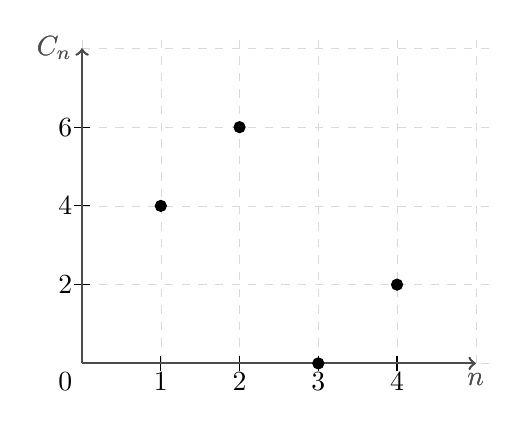
\begin{tikzpicture}
    \draw[help lines, color=gray!30, dashed] (0,0) grid (5.2,4.2);
    \draw[->,thick,black!70] (0,0) -- (5,0) node[below] {$n$}; 
    \draw[->,thick,black!70] (0,0) -- (0,4) node[left] {$C_n$}; 
    \node[below left] at (0,0) {0};
    \foreach \x in {1,2,3,4} \node[below] at (\x,0) {\x};
    \foreach \y in {2,4,6} \node[left] at (0,\y/2) {\y};
    \foreach \x in {1,2,3,4} \draw[-,thin] (\x,-0.1) -- (\x,.1);
    \foreach \y in {1,2,3} \draw[-,thin] (-.1,\y) -- (.1,\y);
    \draw[->,thick,black!70] (0,0) -- (5,0) node[below] {$n$}; 
    \draw[->,thick,black!70] (0,0) -- (0,4) node[left] {$C_n$}; 
    \filldraw[black] (1,2) circle (2pt);
    \filldraw[black] (2,3) circle (2pt);
    \filldraw[black] (3,0) circle (2pt);
    \filldraw[black] (4,1) circle (2pt);
\end{tikzpicture}
\caption{the amplitude spectrum}
\label{fig:fourier_series_single_side_spectrum_example1}
\end{minipage}\hfill
\begin{minipage}[c]{0.47\linewidth}
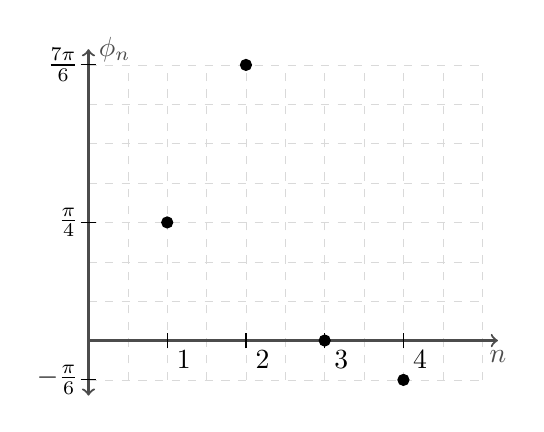
\begin{tikzpicture}
    \draw[help lines, color=gray!30, dashed, step=0.5] (0,0) grid (5,4);
    \draw[->,thick,black!70] (0,0.5) -- (5.2,0.5) node[below] {$n$}; 
    \draw[<->,thick,black!70] (0,-0.2) -- (0,4.2) node[right] {$\phi_n$}; 
    \foreach \x in {1,2,3,4} \node[below right] at (\x,.5) {\x};
    \foreach \x in {1,2,3,4} \draw[-,thin] (\x,.4) -- (\x,.6);
    \foreach \y in {0,2,4} \draw[-,thin] (-.1,\y) -- (.1,\y);
    \node[left] at (0,0) {$-\frac{\pi}{6}$};
    \node[left] at (0,2) {$\frac{\pi}{4}$};
    \node[left] at (0,4) {$\frac{7\pi}{6}$};
    \filldraw[black] (1,2) circle (2pt);
    \filldraw[black] (2,4) circle (2pt);
    \filldraw[black] (3,.5) circle (2pt);
    \filldraw[black] (4,0) circle (2pt);
\end{tikzpicture}
\caption{the phase spectrum}
\label{fig:fourier_series_single_side_spectrum_example2}
\end{minipage}
\end{figure}
% \vspace{25pt}







\subsubsection{Two-Sided Spectra}
From Euler's formula $e^{\mathrm{i}x}=\cos{x}+\mathrm{i}\sin{x}$, we can deduce to get:
\begin{equation}
    \begin{cases}
        \cos(n\omega_0t) = \frac{1}{2}\left[e^{\mathrm{i}n\omega_0t}+e^{-\mathrm{i}n\omega_0t}\right]   \\
        \sin(n\omega_0t) = -\frac{\mathrm{i}}{2}\left[e^{\mathrm{i}n\omega_0t}-e^{-\mathrm{i}n\omega_0t}\right]
    \end{cases}
    \label{equ:cosine_and_sine_in_exponential_form}
\end{equation}
Substitute ({\ref{equ:cosine_and_sine_in_exponential_form}}) into ({\ref{equ:trig_fourier_series_expansion}}), 
we obtain:

$$\begin{aligned} f(t) =& a_0 + 
\sum_{n=1}^{\infty}\frac{a_n}{2}\left[e^{\mathrm{i}n\omega_0t}+e^{-\mathrm{i}n\omega_0t}\right]
+ \sum_{n=1}^{\infty}\frac{b_n}{2\mathrm{i}}\left[e^{\mathrm{i}n\omega_0t}-e^{-\mathrm{i}n\omega_0t}\right] \\
=& a_0 + \sum_{n=1}^{\infty}\left[ \frac{a_n-\mathrm{i}b_n}{2}e^{\mathrm{i}n\omega_0t} 
+ \frac{a_n+\mathrm{i}b_n}{2}e^{-\mathrm{i}n\omega_0t}\right]   \\
=& a_0 + \sum_{n=1}^{\infty}\left[ \frac{a_n-\mathrm{i}b_n}{2}e^{\mathrm{i}n\omega_0t} \right]
+ \sum_{n=-\infty}^{-1}\left[\frac{a_{-n}+\mathrm{i}b_{-n}}{2}e^{\mathrm{i}n\omega_0t}\right]
\end{aligned}$$

By substituting $-n$ into (\ref{equ:trig_fourier_series_cosine_coeff}) and 
(\ref{equ:trig_fourier_series_sine_coeff}), we obtain:
\begin{equation}\begin{cases}
    a_n = a_{-n}    \\
    b_n = -b_{-n}
\end{cases}
\label{equ:coeff_of_negative_n_relationship}
\end{equation}

Let $F_n=\frac{a_n-\mathrm{i}b_n}{2}$, and $F_0=a_0$:

$$\begin{aligned} f(t) =& a_0 + 
    \sum_{n=1}^{\infty}\left[ \frac{a_n-\mathrm{i}b_n}{2}e^{\mathrm{i}n\omega_0t} \right]
    + \sum_{n=-\infty}^{-1}\left[\frac{a_n-\mathrm{i}b_n}{2}e^{\mathrm{i}n\omega_0t}\right] \\
    =& F_0e^{0\mathrm{i}n\omega_0t} + 
    \sum_{n=1}^{\infty}F_ne^{\mathrm{i}n\omega_0t}
    + \sum_{n=-\infty}^{-1}F_ne^{\mathrm{i}n\omega_0t}
\end{aligned}$$

Continue simplifying this equation, we deduced the exponential Fourier Series:
\begin{equation}
    f(t) = \sum_{n=-\infty}^{\infty}F_ne^{\mathrm{i}n\omega_0t}
\end{equation}

Expand $F_n$ with (\ref{equ:trig_fourier_series_cosine_coeff}) and (\ref{equ:trig_fourier_series_sine_coeff}):
$$\begin{aligned} 
    F_n 
    =& \frac{a_n-\mathrm{i}b_n}{2}    \\
    =& \frac{1}{2}\cdot\frac{2}{T} \int_{T} f(t)\cos(n\omega_0t) \mathrm{d}t   
        - \frac{\mathrm{i}}{2}\cdot\frac{2}{T} \int_{T} f(t)\sin(n\omega_0t) \mathrm{d}t
\end{aligned}$$
\indent Apply Euler's formula:
\begin{equation}
    F_n = \frac{1}{T}\int_{T} f(t)e^{-\mathrm{i}n\omega_0t} \mathrm{d}t
    \label{equ:fourier_series_exponent_coeff}
\end{equation}

\indent We had removed another parameter from the equation, combining the amplitudes and phase shifts information 
into a single complex number, $F_n$. The magnitude of $F_n$ describes amplitude, 
and the argument of it describes phase shifts.
Since $F_n = \left|F_n\right|e^{\mathrm{i}\phi_n}$ is a complex number, 
we can calculate the magnitude and argument:

$$\begin{cases}
    \left|F_0\right| = C_0 = D_0  \\
    \left|F_n\right| = \frac{1}{2}\sqrt{a_n^2+b_n^2} = \frac{1}{2}C_n = \frac{1}{2}D_n , n > 0   \\
    \tan(\phi_n) = -\frac{b_n}{a_n} = \tan(\phi_n) = -\cot(\theta_n) , n > 0
\end{cases}$$

\indent Since our Fourier Series included negative values, we can sub in ({\ref{equ:coeff_of_negative_n_relationship}}) 
into the above equation, this suggests that the amplitude, $\left|F_n\right|$ is an even function of $n$, 
while $\phi_n$ is an odd function of $n$. 

$$\begin{cases}
    \left|F_n\right| = \left|F_{-n}\right| \\
    \phi_n = -\phi_{-n}
\end{cases}$$


\noindent\textbf{Example:}

$$f(t) = 4\cos(10\pi t+\frac{\pi}{4}) - 6\cos(20\pi t+\frac{\pi}{6}) + 2\sin(40\pi t+\frac{\pi}{3})$$
\indent Convert the example from the preceding sub-subsection using (\ref{equ:cosine_and_sine_in_exponential_form}):

$$\begin{aligned}
    f(t) 
    =& 4\cos(10\pi t+\frac{\pi}{4}) + 6\cos(20\pi t+\frac{7}{6}\pi) + 2\cos(40\pi t-\frac{\pi}{6})  \\
    =& 2e^{\mathrm{i}\pi(10t+\frac{1}{4})} + 3e^{\mathrm{i}\pi(20t+\frac{7}{6})} + e^{\mathrm{i}\pi(40t-\frac{1}{6})} \\
    &+ 2e^{-\mathrm{i}\pi(10t+\frac{1}{4})} + 3e^{-\mathrm{i}\pi(20t+\frac{7}{6})} + e^{-\mathrm{i}\pi(40t-\frac{1}{6})}
\end{aligned}$$


\indent This also works if $f(t)$ is the sum of sine functions. With the same example, 
since $\cos(x)=\sin(x-\frac{\pi}{2})$, 
we can easily convert all of the cosine terms into sine to use the same example. 
Simply by replacing $-\mathrm{i}$ with 
$e^{\frac{\mathrm{i}\pi}{2}}$ would give the exact same result.

$$\begin{aligned}
    f(t) 
    =& 4\sin(10\pi t+\frac{3\pi}{4}) + 6\sin(20\pi t+\frac{5}{3}\pi) + 2\sin(40\pi t+\frac{\pi}{3}) \\
    =& \mathrm{i}2(e^{-\mathrm{i}\pi(10t+\frac{3}{4})} - e^{\mathrm{i}\pi(10t+\frac{3}{4})}) +
    \mathrm{i}3(e^{-\mathrm{i}\pi(10t+\frac{5}{3})} - e^{\mathrm{i}\pi(20t+\frac{5}{3})}) + \\
    &\hspace{4pc} \mathrm{i}(e^{-\mathrm{i}\pi(40t+\frac{1}{3})} - e^{\mathrm{i}\pi(40t+\frac{1}{3})})       \\
    =& 2(e^{\mathrm{i}\pi(10t+\frac{1}{4})} + e^{-\mathrm{i}\pi(10t+\frac{1}{4})} )
    + 3(e^{\mathrm{i}\pi(20t+\frac{7}{6})} + e^{-\mathrm{i}\pi(20t+\frac{7}{6})})  + \\
    &\hspace{4pc} e^{\mathrm{i}\pi(40t-\frac{1}{6})} + e^{-\mathrm{i}\pi(40t-\frac{1}{6})}
\end{aligned}$$



\begin{figure}[h]
\begin{minipage}[c]{0.47\linewidth}
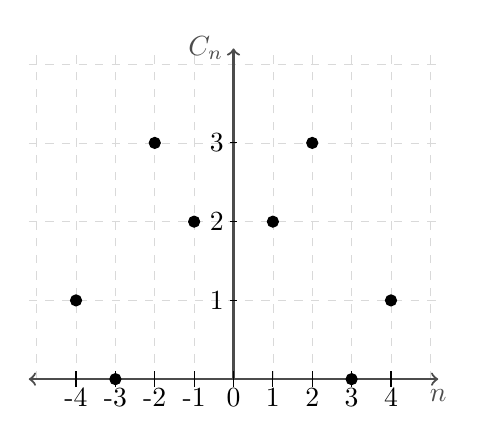
\begin{tikzpicture}[xscale=.5]
    \draw[help lines, color=gray!30, dashed] (-5.2,0) grid (5.2,4.2);
    \draw[<->,thick,black!70] (-5.2,0) -- (5.2,0) node[below] {$n$}; 
    \draw[->,thick,black!70] (0,0) -- (0,4.2) node[left] {$C_n$}; 
    % \node[below left] at (0,0) {0};
    \foreach \x in {-4,-3,-2,-1,0,1,2,3,4} \node[below] at (\x,0) {\x};
    \foreach \y in {1,2,3} \node[left] at (0,\y) {\y};
    \foreach \x in {-4,-3,-2,-1,0,1,2,3,4} \draw[-,thin] (\x,-0.1) -- (\x,.1);
    \foreach \y in {1,2,3} \draw[-,thin] (-.1,\y) -- (.1,\y); 
    \filldraw[black,xscale=2] (.5,2) circle (2pt);
    \filldraw[black,xscale=2] (1,3) circle (2pt);
    \filldraw[black,xscale=2] (1.5,0) circle (2pt);
    \filldraw[black,xscale=2] (2,1) circle (2pt);
    \filldraw[black,xscale=2] (-.5,2) circle (2pt);
    \filldraw[black,xscale=2] (-1,3) circle (2pt);
    \filldraw[black,xscale=2] (-1.5,0) circle (2pt);
    \filldraw[black,xscale=2] (-2,1) circle (2pt);
\end{tikzpicture}
\caption{the amplitude spectrum}
\label{fig:fourier_series_two_side_spectrum_example1}
\end{minipage}\hfill
\begin{minipage}[c]{0.47\linewidth}
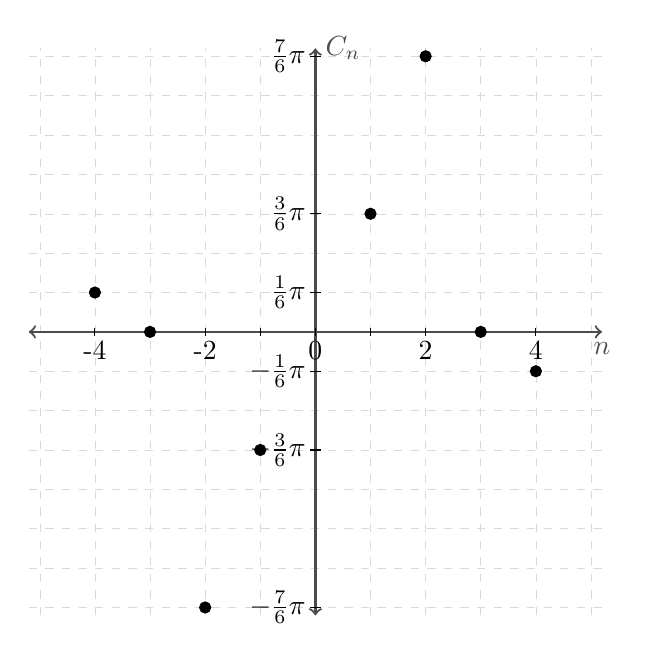
\begin{tikzpicture}[xscale=.7,yscale=.5]
    \draw[help lines, color=gray!30, dashed] (-5.2,-7.2) grid (5.2,7.2);
    \draw[<->,thick,black!70] (-5.2,0) -- (5.2,0) node[below] {$n$}; 
    \draw[<->,thick,black!70] (0,-7.2) -- (0,7.2) node[right] {$C_n$}; 
    % \node[below left] at (0,0) {0};
    \foreach \x in {-4,-2,0,2,4} \node[below] at (\x,0) {\x};
    \foreach \y in {1,3,7} \node[left] at (0,\y) {$\frac{\y}{6}\pi$};
    \foreach \y in {1,3,7} \node[left] at (0,-\y) {$-\frac{\y}{6}\pi$};
    \foreach \x in {-4,-3,-2,-1,0,1,2,3,4} \draw[-,thin] (\x,-0.1) -- (\x,.1);
    \foreach \y in {1,3,7} \draw[-,thin] (-.1,\y) -- (.1,\y);
    \foreach \y in {1,3,7} \draw[-,thin] (-.1,-\y) -- (.1,-\y);
    \filldraw[black,xscale=1/.7,yscale=2] (.7,1.5) circle (2pt);
    \filldraw[black,xscale=1/.7,yscale=2] (1.4,3.5) circle (2pt);
    \filldraw[black,xscale=1/.7,yscale=2] (2.1,0) circle (2pt);
    \filldraw[black,xscale=1/.7,yscale=2] (2.8,-.5) circle (2pt);
    \filldraw[black,xscale=1/.7,yscale=2] (-.7,-1.5) circle (2pt);
    \filldraw[black,xscale=1/.7,yscale=2] (-1.4,-3.5) circle (2pt);
    \filldraw[black,xscale=1/.7,yscale=2] (-2.1,-0) circle (2pt);
    \filldraw[black,xscale=1/.7,yscale=2] (-2.8,.5) circle (2pt);
\end{tikzpicture}
\caption{the phase spectrum}
\label{fig:fourier_series_two_side_spectrum_example2}
\end{minipage}
\end{figure}
\vspace{1pc}

The amplitude spectrum is symmetrical over the $C_n$-axis, while the phase spectrum is a $180^\circ$ rotation.

Comparing these two graphs with the single-sided spectra, 
it is obvious that they look nearly identical for $n \ge 0$. 

If the phase shift is factored out, the function can be expressed with only the amplitudes; however, the amplitude becomes a complex number:
$$\begin{aligned}
    f(t) 
    =& 2(e^{\mathrm{i}\pi(10t+\frac{1}{4})} + e^{-\mathrm{i}\pi(10t+\frac{1}{4})} )
    + 3(e^{\mathrm{i}\pi(20t+\frac{7}{6})} + e^{-\mathrm{i}\pi(20t+\frac{7}{6})})  + \\
    &\hspace{4pc} e^{\mathrm{i}\pi(40t-\frac{1}{6})} + e^{-\mathrm{i}\pi(40t-\frac{1}{6})} \\ 
    =& 2e^{\mathrm{i}\frac{\pi}{4}}e^{\mathrm{i}10\pi t} + 2e^{-\mathrm{i}\frac{\pi}{4}}e^{-\mathrm{i}10\pi t} 
    + 3e^{\mathrm{i}\frac{7\pi}{6}}e^{\mathrm{i}20\pi t} + 3e^{-\mathrm{i}\frac{7\pi}{6}}e^{-\mathrm{i}20\pi t}  + \\
    &\hspace{4pc} e^{-\mathrm{i}\frac{\pi}{6}}e^{\mathrm{i}40\pi t} + e^{\mathrm{i}\frac{\pi}{6}}e^{-\mathrm{i}40\pi t} \\
\end{aligned}$$

% \begin{tabularx}{0.8\textwidth} { 
%   | >{\raggedright\arraybackslash}X 
%   | >{\centering\arraybackslash}X 
%   | >{\raggedleft\arraybackslash}X | }
\renewcommand{\arraystretch}{2}
\noindent
\begin{center}
\begin{tabularx}{\textwidth}
{ |c||>{\centering\arraybackslash}X|>{\centering\arraybackslash}X|>{\centering\arraybackslash}X|>{\centering\arraybackslash}X|>{\centering\arraybackslash}X|>{\centering\arraybackslash}X|>{\centering\arraybackslash}X|>{\centering\arraybackslash}X|>{\centering\arraybackslash}X| }
 \hline
 $n$ & -4 & -3 & -2 & -1 & 0 & 1 & 2 & 3 & 4 \\
 \hline
 $C_n$ & $e^{\frac{\pi}{6}\mathrm{i}}$ & 0 & $3e^{-\frac{7\pi}{6}\mathrm{i}}$ & $2e^{-\frac{\pi}{4}\mathrm{i}}$ & 0 & $2e^{\mathrm{i}\frac{\pi}{4}}$ & $3e^{\frac{7\pi}{6}\mathrm{i}}$ & 0 & $e^{-\frac{\pi}{6}\mathrm{i}}$ \\
\hline
\end{tabularx}
\end{center}
